\section{Příklad 2}
% Jako parametr zadejte skupinu (A-H)
\druhyZadani{E}

Upravíme zapojení:
    \begin{figure}[ht]
		\begin{center}
			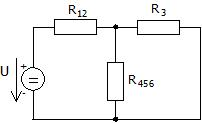
\includegraphics[width=5cm,keepaspectratio]{fig/Pr2_1_2019.jpeg}
		\end{center}
	\end{figure}
	
    \begin{eqnarray*}
        R_{12} &= & R_{1} + R_{2} = 150 + 335 = 485 \Omega\\
	\end{eqnarray*}

Vypočítáme nové konstanty:
    \begin{figure}[ht]
		\begin{center}
			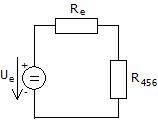
\includegraphics[width=4cm,keepaspectratio]{fig/Pr2_2_2019.jpeg}
		\end{center}
	\end{figure}
	
    \begin{eqnarray*}
        R_{e} &= & \frac{R_{12} * R_{3}}{R_{12} + R_{3}} = \frac{485 * 625}{485 + 625} = 273.0856 \Omega\\
        U_{e} &= & U * \frac{R_{3}}{R_{12} + R_{3}} = 250 * \frac{625}{485 + 625} = 140.7658 V\\
	\end{eqnarray*}
	
\pagebreak
Zpětně upravíme zapojení:
    \begin{figure}[ht]
		\begin{center}
			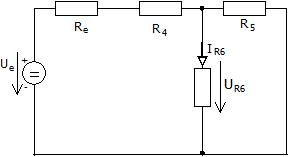
\includegraphics[width=7cm,keepaspectratio]{fig/Pr2_3_2019.jpeg}
		\end{center}
	\end{figure}

Zjednodušíme zapojení:
    \begin{figure}[ht]
		\begin{center}
			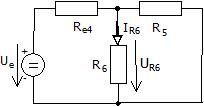
\includegraphics[width=5cm,keepaspectratio]{fig/Pr2_4_2019.jpeg}
		\end{center}
	\end{figure}
    \begin{eqnarray*}
        R_{e4} &= & R_{e} + R_{4} = 273.0856 + 245 = 518.0856 \Omega\\
	\end{eqnarray*}

Opět vypočítáme nové konstanty:
    \begin{figure}[ht]
		\begin{center}
			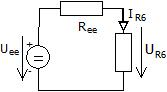
\includegraphics[width=4cm,keepaspectratio]{fig/Pr2_5_2019.jpeg}
		\end{center}
	\end{figure}
    \begin{eqnarray*}
        R_{ee} &= & \frac{R_{e4} * R_{5}}{R_{e4} + R_{5}} = \frac{518.0856 * 600}{518.0856 + 600} = 278.0211 \Omega\\
        R_{ee6} &= & R_{ee} + R_{6} = 278.0211 + 150 = 428.0211 \Omega\\
        U_{ee} &= & U_{e}*\frac{R_{5}}{R_{e4} + R_{5}} = 140.4658 * \frac{600}{518.0856 + 600} = 75.5394 V\\
        I_{ee} &= & \frac{U_{ee}}{R_{ee6}} = \frac{75.5394}{428.0211} = 0.1765 A\\
	\end{eqnarray*}
	
Výpočítáme hledané hodnoty:
    \begin{eqnarray*}
        U_{R6} &= & U_{ee} - R_{ee} * I_{ee} = 75.5394 - 278.0211 * 0.1765 = 26.4687 V\\
        I_{R6} &= & \frac{U_{R6}}{R_{6}} = \frac{26.4687}{150} = 0.1765 A\\
	\end{eqnarray*}

Hledané hodnoty $U_{R6}$ a $I_{R6}$ jsou:
    \begin{eqnarray*}
        U_{R6} &= & 26.4687 V\\
        I_{R6} &= & 0.1765 A\\
	\end{eqnarray*}